\chapter{LE2ML: un \textit{workbench} modulaire pour l'apprentissage machine}
\label{chap:6}

% Grâce aux chapitres précédents, il a été montré que les \textit{wearable devices} sont de plus en plus utilisés dans le processus de reconnaissance d'activités au sein des habitats intelligents. Aussi, ces dispositifs ont également été employés dans l'objectif de répondre à plusieurs autres problématiques relatives à l'assistance des résidents de ces habitats, au sens large. Néanmoins, l'engouement croissant pour les \textit{wearable devices} a permis d'identifier plusieurs problématiques quant à leur utilisation dans ce contexte de recherche particulier. En effet, il a été évalué que la plupart des différentes architectures d'habitats intelligents qui ont été proposées n'ont pas été conçues dans une optique évolutive. Ainsi, celles-ci ne permettent pas d'y intégrer de manière rapide et efficace de nouveaux capteurs, comme les \textit{wearable devices}, ou de nouveaux composants logiciels pour effectuer le processus de reconnaissance d'activités et l'assistance aux résidents.

% Pour ce travail, l'intégration des \textit{wearable devices} dans les architectures de maisons intelligentes s'est concentrée avant tout sur l'aspect logiciel plutôt que matériel, dans la conception des méthodes de reconnaissance que ces dispositifs proposent. En effet, tout comme pour la reconnaissance d'activités réalisée de manière classique, c'est-à-dire, en exploitant les capteurs et effecteurs ambiants présents dans l'habitat, les différents processus proposés par les dispositifs sont, dans une vaste majorité des cas, encapsulés au sein d'un unique composant logiciel immuable. De la même manière, la réutilisation de mécanismes communs, le déploiement de ces méthodes et leur modification demeurent alors des tâches complexes à mettre en \oe{}uvre.

% Malgré cela, certains travaux ont fait mention de l'emploi d'un \textit{workbench} d'apprentissage machine afin de traiter les données produites par les \textit{wearable devices} et de réaliser la reconnaissance d'activité \citep{Chapron2018}. D'un point de vue académique, ces outils ne sont pas nouveaux et ils permettent un prototypage rapide, la visualisation des données ainsi qu'une meilleure reproductibilité des méthodes expérimentales et une meilleure réutilisation des composants logiciels \citep{Holmes1994,Langlois2008}. À titre d'exemple, l'outil le plus connu et le plus répandu dans la littérature est \acs{WEKA}. Il s'agit d'un \textit{workbench} open source issue de la recherche académique qui supporte un grand nombre d'algorithmes d'apprentissage machine supervisés et non supervisés \citep{Witten2016}. Celui-ci a été utilisé en tant que librairie dans la méthode de reconnaissance des types de sols présentée au Chapitre \ref{chap:4}. Néanmoins, bien que ce \textit{workbench} offre un large éventail d'options, son utilisation reste relativement gourmande en termes d'utilisation des ressources de calcul et de mémoire. De plus, les fonctionnalités offertes par cet outil demeurent particulièrement contraignantes à étendre et, en raison de sa conception, il n'est pas particulièrement adapté pour être utilisé dans l'architecture d'habitats intelligents distribuée qui a été introduite dans le chapitre précédent.

% Ainsi, ce dernier travail présente \acs{LE2ML} (\acl{LE2ML}), un nouveau type de \textit{workbench} pour l'apprentissage machine qui repose sur l'utilisation de microservices. De la même manière que pour l'implémentation de l'architecture proposée, cette conception logicielle a été choisie, car la technologie des microservices permet une meilleure évolutivité, des déploiements plus sûrs et plus rapides ainsi qu'une meilleure isolation des pannes \citep{Dragoni2017}. Cependant, l'avantage principal d'une telle conception concerne l'aspect modulaire que permettent les microservices. Ainsi, ce \textit{workbench} demeure un outil agnostique, tant en termes de langages de programmation que de plateformes supportées, qui peut être déployé dans n'importe quel environnement, et ce, sans aucune contrainte complexe.

\hl{Dans le chapitre précédent, une nouvelle architecture d'habitat intelligent a été présentée. Dans sa conception, cette implémentation suggère de s'appuyer sur la technologie des microservices puisque ceux-ci offrent un meilleur niveau de flexibilité et de modularité. Ainsi, cette technologie permet donc d'abstraire le type de capteurs (ambiants ou \textit{wearable devices}) qui est utilisé pour le processus de reconnaissance d'activités. Cependant, pour réaliser la reconnaissance d'activités avec des \textit{wearable devices}, la plupart des méthodes actuellement proposées sont des applications complètes. Par conséquent, les différents processus qui composent la reconnaissance sont, la plupart du temps, encapsulés au sein d'un unique composant logiciel immuable. Il devient donc difficile de les modifier. De plus, le fait de disposer d'une unique application ne favorise pas la réutilisation de certains mécanismes communs à plusieurs méthodes. Ceux-ci doivent donc généralement être soit développés à nouveau, soit adaptés afin de pouvoir supporter des modifications dans la méthode proposée. De surcroît, l'exploitation de ce genre d'application} \og \hl{prête à l'emploi} \fg \hl{est, la plupart du temps, complexifiée. En effet, selon les dépendances, le langage de programmation et la plateforme, elles peuvent être difficiles à adapter et à déployer d'un environnement à un autre (\textit{p. ex.} entre deux laboratoires de recherche différents). De ce fait, la question de recherche qui est spécifiquement examinée dans ce chapitre est : \textit{\og comment prendre en considération la diversité des composants logiciels, et plus précisément, ceux exploités par les \textit{wearable devices}, qui composent les différents processus d'apprentissage en facilitant leur intégration, leur réutilisation ainsi que leur déploiement au sein de l'architecture ? \fg}}

\hl{Pour répondre à cette question, ce chapitre présente} \acs{LE2ML} (\acl{LE2ML})\hl{, un nouveau type de \textit{workbench} pour l'apprentissage machine qui repose sur l'utilisation de microservices établis par l'architecture introduite au chapitre précédent. De la même manière, cette conception logicielle a été choisie, }car la technologie des microservices permet une meilleure évolutivité, des déploiements plus sûrs et plus rapides ainsi qu'une meilleure isolation des pannes \citep{Dragoni2017}. Cependant, l'avantage principal de cette solution concerne l'aspect modulaire que permettent les microservices. \hl{De plus, le souhait de proposer une telle conception a été amplifié par la volonté de finaliser l'intégration logicielle des \textit{wearable devices} au sein de l'architecture en \textit{cluster} présentée précédemment. Cependant, puisque ce \textit{workbench} demeure un outil agnostique, tant en termes de langages de programmation que de plateformes supportées, qui peut être déployé dans n'importe quel environnement, et ce, sans aucune contrainte complexe; les habitats intelligents qui n'exploitent pas les \textit{wearable devices} pourraient malgré tout tirer profit d'une telle solution.}

\hl{La suite de ce chapitre commence par présenter le fonctionnement du \textit{workbench}} \acs{LE2ML}\hl{. Ensuite,} une expérimentation pour évaluer la reproductibilité de l'expérimentation proposée dans le Chapitre \ref{chap:4} et valider les résultats attendus est décrite dans une troisième section. Finalement, dans une dernière partie, ce chapitre dresse une conclusion quant à ce dernier travail.

\section{Solution proposée}

\hl{Dans le Chapitre} \ref{chap:2}\hl{, les trois principaux \textit{workbench} d'apprentissage machine ont été présentés dans le but de déterminer les problématiques de chacune de ces solutions. Ainsi, il a été montré que tous ces outils présentent le même principal inconvénient, c'est-à-dire, une forte dépendance à leur contexte d'utilisation.} En effet, bien que toutes ces solutions permettent d'intégrer des composants logiciels personnalisés, ceux-ci doivent être conçus pour répondre aux exigences de l'outil pour lequel ils sont développés. De plus, dans un contexte de recherche académique, ces paquets additionnels peuvent devenir difficiles à maintenir. En effet, ils doivent être installés manuellement sur chacun des dispositifs qui composent l'environnement (\textit{p. ex.} ordinateurs ou serveurs), ce qui provoque indubitablement des problèmes de déploiement et de réutilisation.

\hl{Par conséquent,} ce chapitre présente \acs{LE2ML}\footnote{\url{https://github.com/FlorentinTh/LE2ML}} (\acl{LE2ML}), un nouveau type de \textit{workbench} d'apprentissage machine qui, comme pour l'architecture introduite précédemment, s'appuie sur la technologie des microservices. Bien que cet outil ait été spécifiquement conçu pour être utilisé dans notre architecture, il est parfaitement possible de le faire fonctionner dans des environnements plus traditionnels tels qu'un serveur dans une architecture de maison intelligente monolithique ou un simple ordinateur. La seule contrainte préalable est d'y installer le moteur de conteneurs Docker. LE2ML a été développé dans le but d'être modulaire. De ce fait, le composant principal de la conception de son architecture logicielle est une \acs{API} (\acl{API}) \acs{REST}. Cette API est principalement chargée de piloter tous les autres composants logiciels du \textit{workbench} qui sont considérés comme des modules que n'importe qui peut développer afin d'intégrer à l'outil de nouvelles fonctionnalités selon les besoins. Enfin, une application web a également été développée pour faciliter les interactions avec l'\acs{API}. La Figure \ref{fig:containers_workbench} présente un exemple de déploiement possible pour \acs{LE2ML}. En effet, celle-ci illustre l'organisation des conteneurs et de leurs réseaux superposés qui sont nécessaires pour que le \textit{workbench} fonctionne sur notre architecture. Ainsi, cette figure va guider les explications fournies dans le reste de ce chapitre.

\begin{figure}[H]
	\centering
	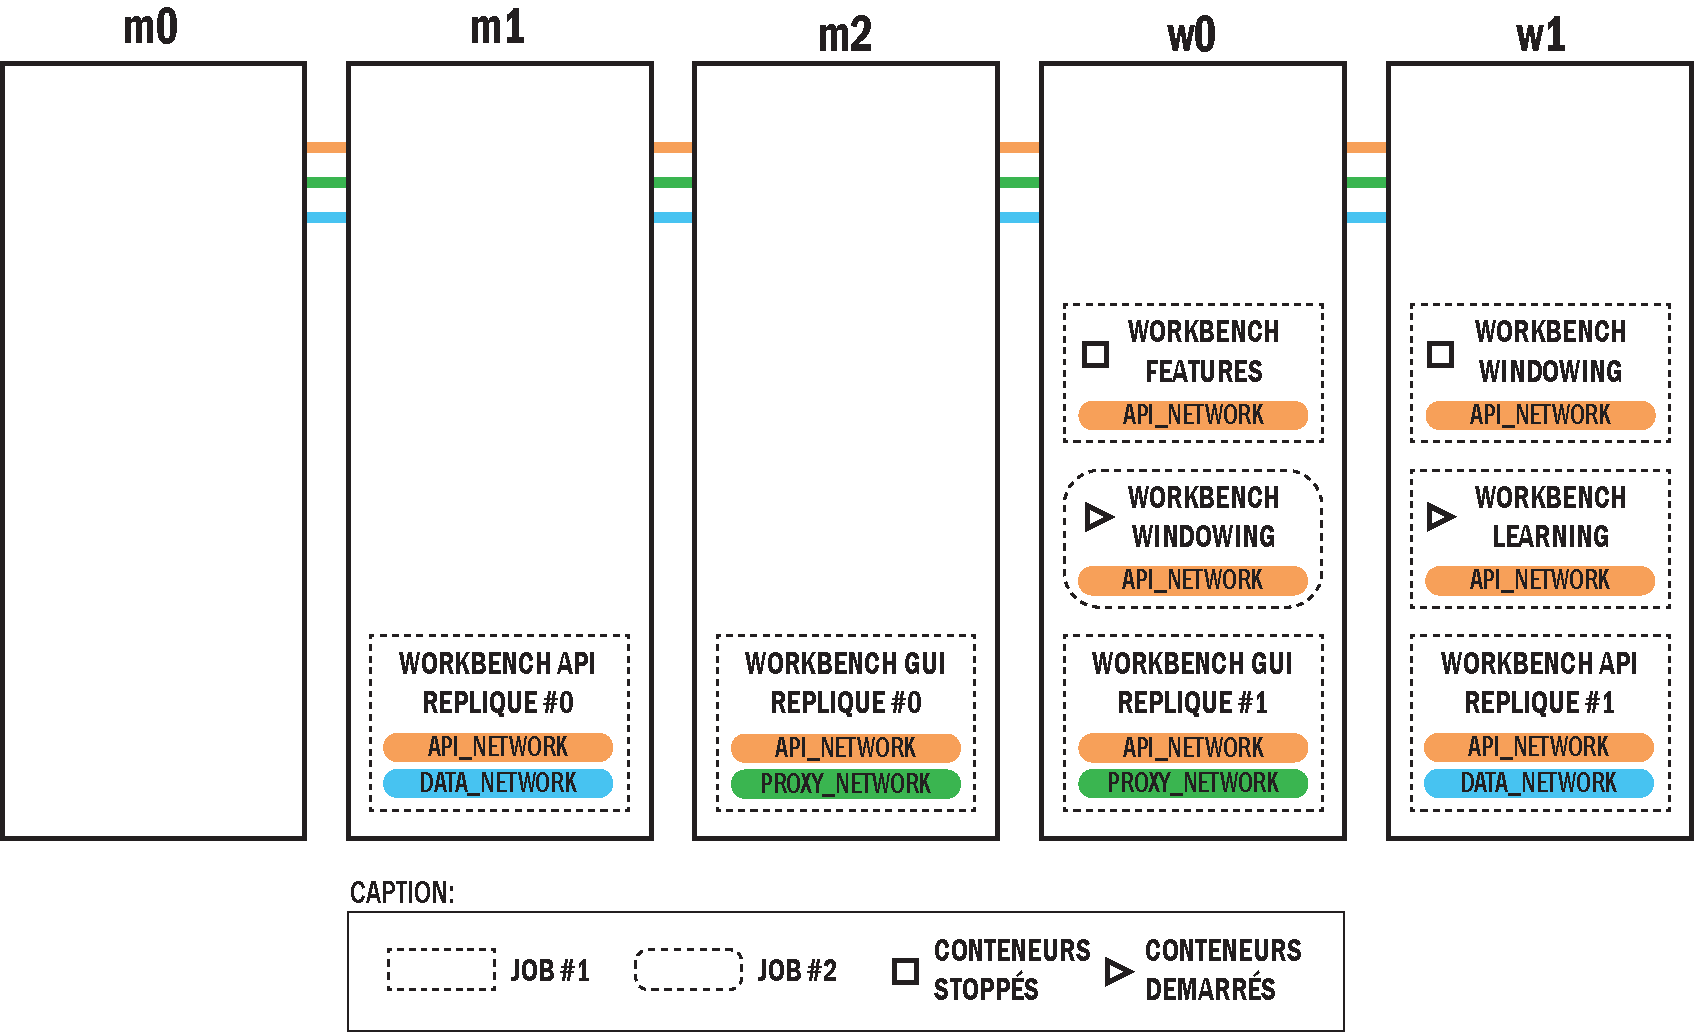
\includegraphics[width=.9\linewidth]{chapter6/containers_workbench.pdf}
        \caption{Exemple de placement des conteneurs et leurs réseaux superposés sur chaque n\oe{}ud de l'architecture proposée précédemment lors du déploiement de \acs{LE2ML}.}
	\label{fig:containers_workbench}
\end{figure}

\subsection{\acs{API} \acs{REST}}

En tant que composant logiciel principal dans la conception de \acs{LE2ML}, l'\acs{API}\footnote{\url{https://github.com/FlorentinTh/LE2ML-API}}, a été développée grâce à Node.js\footnote{\url{https://nodejs.org}}. Cet outil constitue un environnement d'exécution basée sur le moteur V8\footnote{\url{https://v8.dev}} qui permet de créer des applications côté serveur en JavaScript. Ensuite, le \textit{framework} Express.js\footnote{\url{https://expressjs.com}} a également été employé pour la création de l'\acs{API} \acs{REST}. Plus précisément, celui-ci a permis de simplifier la définition des fonctions de traitement associées aux requêtes \acs{HTTP} qui répondent aux différentes \acs{URI} de l'application (cf. Section \ref{sec:services_web}).

Par ailleurs, comme le montre la Figure \ref{fig:containers_workbench}, cette \acs{API} a été déployée en tant que service utilisant deux répliques. Celles-ci peuvent être exécutées soit sur des n\oe{}uds de type \textit{manager} ou sur des \textit{workers}. Cet exemple de déploiement demeure la recommandation suggérée puisque l'accessibilité de l'\acs{API} est garantie, même en cas de défaillance d'un n\oe{}ud de l'architecture. Toutefois, en fonction de la demande en ressource, c'est-à-dire, lorsque l'\acs{API} doit traiter un grand nombre de requêtes qui sont produites par plusieurs utilisateurs, il est possible de procéder à une mise à l'échelle du service afin d'éviter un ralentissement de l'ensemble du \textit{workbench}. De plus, bien que le service de l'\acs{API} fournisse son propre réseau superposé (\texttt{api\_network}), l'ensemble de ses répliques doivent aussi être relié au réseau de données (\texttt{data\_network}) afin de pouvoir communiquer avec la base de données déployée au sein de l'architecture. En effet, l'\acs{API} doit principalement être en mesure de manipuler les données relatives aux utilisateurs, tâches et sources de données, mais également aux algorithmes d'apprentissage machine, de fenêtrage et d'extraction de caractéristiques qui sont utilisés dans les modules de \acs{LE2ML}. Bien que cette implémentation a été préférée dans le cadre d'une utilisation avec l'architecture présentée dans le chapitre précédent, la mise à disposition d'une base de données non relationnelle n'est cependant pas une contrainte imposée pour assurer le fonctionnement du \textit{workbench} dans des environnements différents.

L'objectif principal de l'\acs{API} de \acs{LE2ML} est d'exécuter plusieurs processus (\emph{jobs}) d'apprentissage machine simultanés grâce à la définition de \textit{pipelines} pour ce processus. Pour ce faire, l'\acs{API} est chargée d'orchestrer le démarrage des différents modules du \textit{workbench} qui s'exécutent alors à l'intérieur de conteneurs. Lorsque tous les modules ont terminé, le \textit{pipeline} d'apprentissage machine est complété et la performance de la reconnaissance est donnée selon plusieurs métriques d'évaluation. De plus, l'\acs{API} propose également plusieurs fonctionnalités de base qui ne sont pas des modules, car elles sont complémentaires au processus d'apprentissage machine. Celles-ci comprennent l'importation de fichiers de données, la gestion de ces fichiers importés ou nouvellement créés, la visualisation des données, la gestion de l'authentification et des autorisations pour les utilisateurs et les applications, la gestion des utilisateurs et de leur rôle ainsi que la gestion des modules.

La définition d'un \textit{pipeline} d'apprentissage machine se fait par le biais d'un fichier \ac{YAML}. Cette approche a été choisie, car un tel type de fichier demeure plus facile à lire et à écrire que le format \acs{JSON}. Par ailleurs, le \acs{YAML} est un format qui se prête particulièrement bien avec l'utilisation de systèmes de gestion de versions (\aclp{VCS} ou \acsp{VCS}) pour être partagés entre plusieurs expérimentateurs au sein d'une équipe de recherche. Une fois transmis à l'\acs{API}, le fichier de définition du \textit{pipeline} est converti en format JSON afin d'être validé grâce à un schéma, puis il est stocké sur le système de fichiers distribué. Ensuite, le contenu du fichier est analysé par l'\acs{API} afin que toutes les tâches qui composent le \textit{pipeline} soient lancées de manière consécutive. Un exemple d'un tel fichier de définition est présenté en Figure \ref{fig:pipeline_conf}.

\begin{figure}[H]
	\centering
	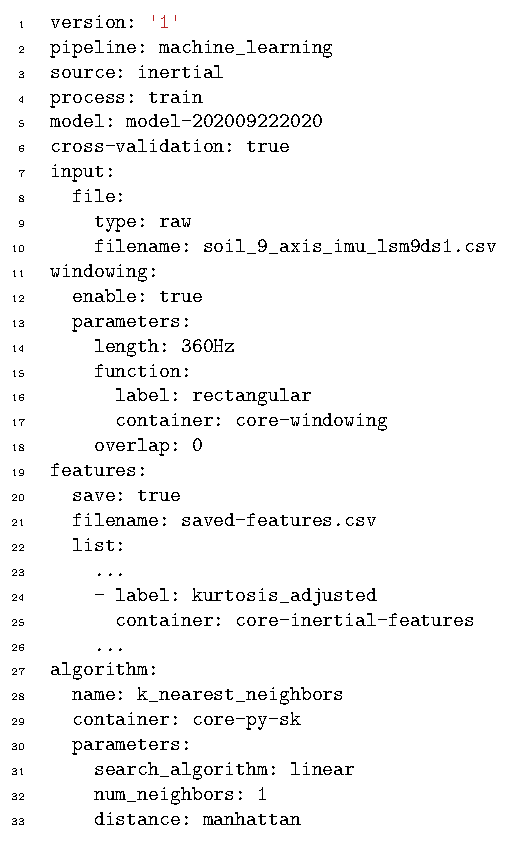
\includegraphics[width=.45\linewidth,keepaspectratio]{chapter6/pipeline_conf.pdf}
        \caption{Exemple d'un fichier de définition d'un \textit{pipeline} qui décrit la phase d'entraînement d'un processus d'apprentissage machine traditionnel.}
	\label{fig:pipeline_conf}
\end{figure}

Dans un premier temps, l'utilisateur doit préciser le type de \textit{pipeline} qui doit être réalisé. Les possibilités sont soit apprentissage machine (\texttt{machine\_learning}), soit apprentissage profond (\texttt{deep\_learning}). Une autre propriété obligatoire concerne la source de données. Celle-ci correspond au type de données qui sont traitées au cours du processus (\textit{p. ex.} des données inertielles ou vocales). Par ailleurs, lorsqu'il s'agit d'un \textit{pipeline} définissant un processus d'apprentissage machine traditionnel, la propriété \texttt{process} doit également être déclarée. Les valeurs possibles sont \texttt{train} et \texttt{test} qui font respectivement référence aux phases d'entraînement et de test pour un tel processus. Il est également possible d'y attribuer la valeur \texttt{none}\textemdash ceci dans le but de permettre aux utilisateurs de réaliser uniquement certaines tâches qui précèdent le processus d'apprentissage, comme l'extraction de caractéristiques. Comme le montre cet exemple, dans le cas où le \textit{pipeline} doit accomplir une phase d'entraînement, l'attribut \texttt{model} doit obligatoirement être fourni. Ainsi, le modèle de données qui a été entrainé par l'algorithme d'apprentissage est sauvegardé sur le système de fichier pour être réutilisé ultérieurement (\textit{p. ex.} lors de la définition d'une phase de prédiction). De plus, la propriété \texttt{cross-validation} est la dernière propriété imposée lorsqu'il s'agit d'une phase d'entraînement. Elle permet de produire une estimation des performances de reconnaissance en évaluant le modèle nouvellement créé grâce à la méthode de la validation croisée en 10 plis.

Ensuite, il est nécessaire de déclarer les données d'entrée sur lesquelles est appliqué le processus d'apprentissage machine. Actuellement, seules deux options sont autorisées, à savoir, la définition d'un fichier ou une connexion WebSocket. Lorsqu'il s'agit d'une source d'entrée de type WebSocket, l'\acs{URL} du serveur doit être indiquée. Sinon, les fichiers doivent être référencés selon leur nom et le type de données qu'ils contiennent (\textit{p. ex.} données brutes : \texttt{raw}). Enfin, le reste du contenu du fichier permet de décrire les différentes tâches et leurs paramètres associés qui sont utilisés lors de l'exécution des modules.

Pour compléter l'exécution des \emph{jobs}, l'\acs{API} a la responsabilité de démarrer les conteneurs selon la définition des tâches fournie dans les fichiers de définition de \textit{pipelines}. Ainsi, puisque certains conteneurs dépendent du résultat de la tâche précédente, ils sont, pour un \emph{job} donné, lancés les uns après les autres. Néanmoins, lorsqu'une même tâche est définie pour utiliser plusieurs conteneurs distincts, ceux-ci sont démarrés en même temps. Ils s'exécutent alors en parallèle. Enfin, les \emph{jobs} qui sont créés par les différents utilisateurs du \textit{workbench} sont également exécutés en parallèle. Ceux-ci sont aussi indépendants les uns des autres bien qu'ils utilisent des images de conteneurs identiques. À titre d'exemple, la Figure \ref{fig:containers_workbench} montre deux \emph{jobs} démarrés à des moments différents, mais dont le traitement est concurrent. En effet, il est possible d'observer que pour le premier \emph{job}, les tâches de fenêtrage et d'extraction de caractéristiques sont toutes les deux terminées alors que le conteneur d'apprentissage est toujours en cours d'exécution. À l'inverse, la tâche de fenêtrage pour le second \emph{job} vient juste de commencer et les autres conteneurs ne sont pas visibles, car ils n'ont pas encore été démarrés.

Pour qu'un conteneur devienne un module de \acs{LE2ML}, trois variables d'environnement doivent être définies, lors de son lancement. Il s'agit de l'identifiant unique du \emph{travail}, de l'identifiant unique de l'utilisateur ainsi que d'un jeton unique généré aléatoirement pour chaque conteneur. Le jeton est utilisé pour permettre à l'\acs{API} de faire le lien entre un conteneur en particulier et la tâche à laquelle il est rattaché. Par conséquent, il est possible de mettre à jour l'entrée du \emph{job} associé dans la base de données. En effet, une fois son traitement terminé, un module LE2ML doit communiquer son état (succès ou échec) à l'\acs{API} par le biais d'un \textit{endpoint} prévu à cet effet. De telles requêtes ne sont permises que si les conteneurs y sont autorisés. Cette vérification est établie grâce à une clé d'application générée au préalable pour chaque application.

Finalement, comme l'exécution des processus d'apprentissage machine implique la création de fichiers, ces informations résultantes du traitement de chaque tâche du \textit{pipeline} sont écrites sur le système dans des dossiers séparés par \emph{job}. En ce sens, ces dossiers sont montés en tant qu'espaces de travail pour tous les conteneurs définis pour un \emph{job} donné.

\subsection{Application Web}

Pour faciliter l'interaction avec l'\acs{API}, nous avons jugé approprié de proposer une interface. De ce fait, une interface graphique\footnote{\url{https://github.com/FlorentinTh/LE2ML-GUI}} a été préférée à une interface de type \acs{CLI} (dont le développement n'est pas exclu dans un avenir proche). En effet, puisque les équipes de recherche sont, la plupart du temps, multidisciplinaires, la conception d'une \acs{GUI} a été priorisée, car ce type d'interface est plus simple à apprendre et à utiliser pour les utilisateurs néophytes. Cette application web a été développée grâce à des technologies modernes. En effet, sa conception repose principalement sur un \textit{framework} JavaScript qui supporte ECMAScript 6 et les versions supérieures de ce standard (ES6+). Celui-ci a été développé spécifiquement pour les besoins de cette application. Par ailleurs, la stratégie de déploiement qui a été adoptée pour ce composant applicatif demeure la même que pour l'\acs{API}, c'est-à-dire, un service répliqué admettant deux instances qui peuvent être placées soit sur un n\oe{}ud \textit{manager}, soit sur un \textit{worker}.

La Figure \ref{fig:le2ml_gui} montre une capture d'écran de la vue principale de l'interface qui permet de créer des \textit{jobs} d'apprentissage machine. Le fil d'Ariane (\texttt{A}) permet d'indiquer aux utilisateurs les étapes qui doivent être complétées pour définir toutes les tâches du \textit{pipeline}. Dans une vue précédente à cette capture d'écran, l'utilisateur doit sélectionner le type d'apprentissage machine qu'il souhaite réaliser (dans le cas présent, il s'agit d'un apprentissage machine traditionnel). Pour chaque étape du \textit{pipeline}, un ensemble de composants web (\texttt{B}) est proposé pour permettre aux utilisateurs de configurer chaque tâche de manière pratique. Cependant, bien qu'il soit possible de construire les fichiers de définition en interagissant avec l'interface graphique, une fonction d'import (\texttt{C}) a également été prévue pour permettre la réutilisation des définitions de \textit{pipeline} existantes. Dans ce contexte, les composants web pour chacune des étapes sont préremplis en fonction du contenu du fichier téléchargé.

\begin{figure}[H]
	\centering
	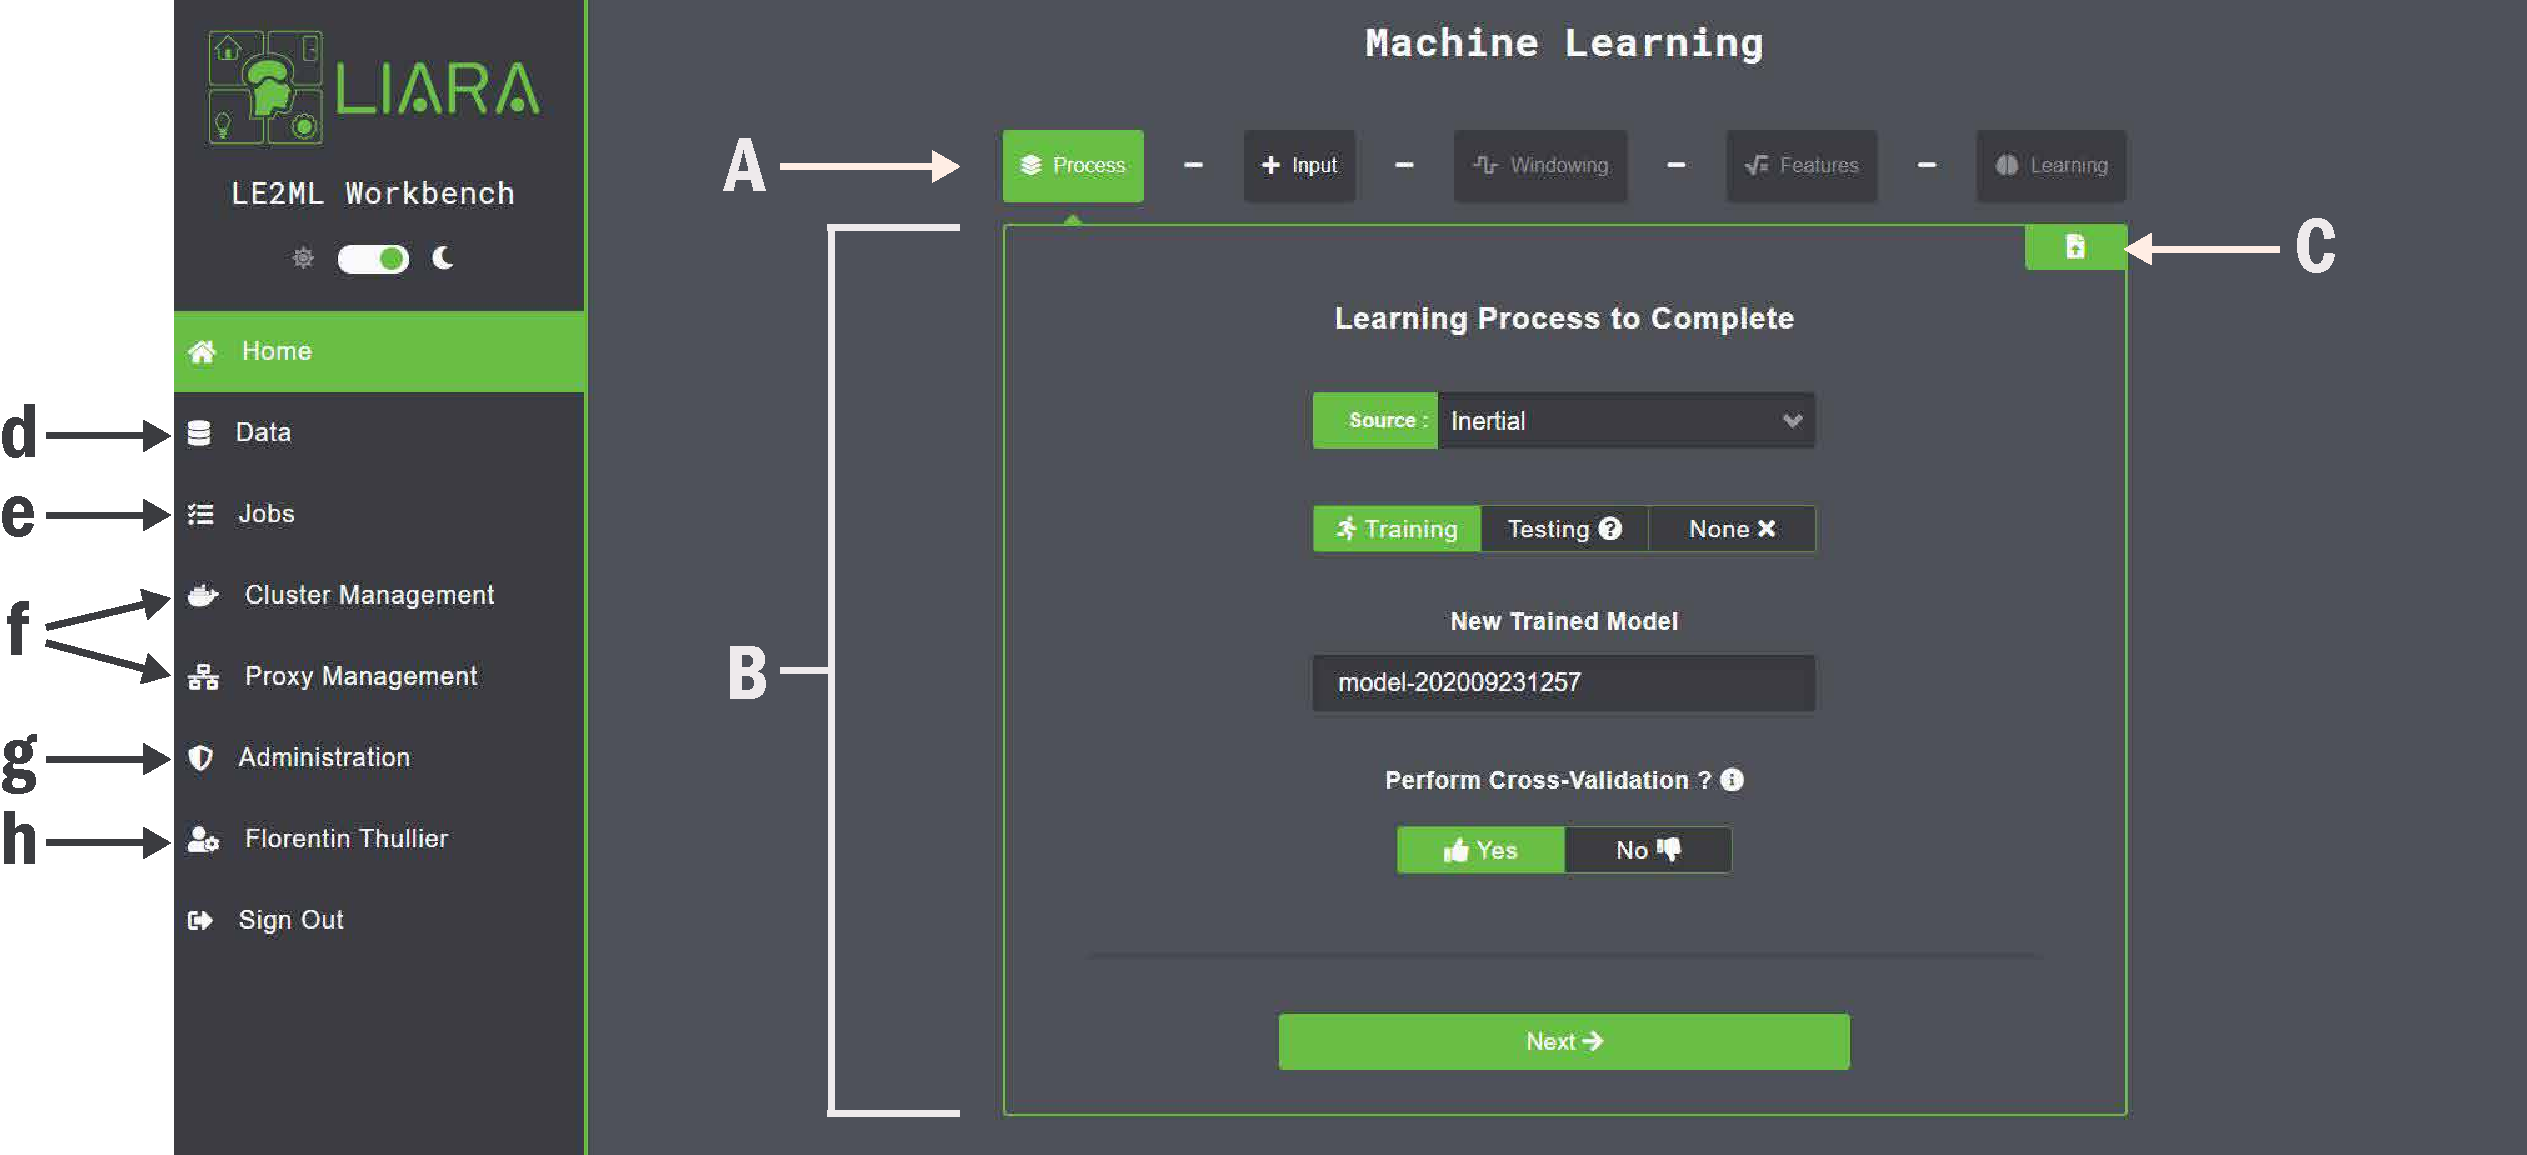
\includegraphics[angle=90,origin=c,height=.85\textwidth,keepaspectratio]{chapter6/le2ml_gui.pdf}
        \caption{Capture d'écran de l'application web qui montre la première étape de la définition d'un \textit{pipeline} d'apprentissage machine.}
	\label{fig:le2ml_gui}
\end{figure}

Par ailleurs, cette interface offre également aux utilisateurs un moyen d'interagir avec toutes les autres fonctionnalités de l'\acs{API}. Le menu \textit{Data} (\texttt{d}) regroupe toutes les fonctionnalités liées aux fichiers de données d'entrée. Celles-ci comprennent un composant pour téléverser de nouveaux fichiers, une vue permettant de naviguer dans le système de fichiers distribué, un outil de visualisation des données ainsi qu'un accès aux différents modules de prétraitement et de fusion des données. Le menu \textit{Jobs} (\texttt{e}) présente la liste des \textit{jobs} d'apprentissage machine en cours de traitement et terminés qui ont été créés par l'utilisateur connecté. Cette liste est mise à jour en temps réel grâce à la technologie \ac{SSE} qui permet à l'\acs{API} d'envoyer des notifications \textit{push} à l'application web. Par le biais de cette vue, il est également possible de télécharger les fichiers résultant d'un \textit{job} complété. Ces fichiers peuvent être soit un rapport comprenant des mesures d'évaluation de la performance qui sont calculées pendant la phase d'entraînement, soit la liste des prédictions déterminées lors de la phase de test. Ensuite, les menus \textit{Cluster Management} et \textit{Proxy Management} (\texttt{f}) redirigent vers les tableaux de bord de Portainer et de Tr\ae{}fik respectivement. Le menu \textit{Administration} (\texttt{g}) permet aux utilisateurs qui ont le rôle administrateur de gérer les modules, les clés d'application ainsi que les utilisateurs inscrits. Enfin, les utilisateurs connectés ont également accès à leur profil (\texttt{i}), où il leur est possible de modifier la plupart de leurs informations personnelles, y compris leur mot de passe.

\subsection{Modules proposés}

Dans la mesure où \acs{LE2ML}, de par sa conception, a pour objectif de fournir une meilleure flexibilité, plusieurs modules ont été conçus pour réaliser certaines tâches spécifiques qui composent le processus d'apprentissage machine. Leur développement a été simplifié afin que quiconque soit capable d'étendre les fonctionnalités du \textit{workbench} en proposant ses propres mécanismes. Ainsi, il est possible de proposer des modules pour le traitement de données telles que les méthodes de prétraitement ou de fusion de données, mais également, des modules qui proposent de nouvelles techniques d'extraction de caractéristiques ou de nouveaux algorithmes d'apprentissage machine.

Le premier avantage principal qui motive l'usage de modules est qu'ils fournissent un moyen simple de pallier la diversité dans la conception de logiciels, tant en termes de langages de programmation, que d'environnements d'exécution qui forment le vaste monde des techniques liées au processus d'apprentissage machine. Par exemple, lorsque des chercheurs développent de nouveaux algorithmes, ces derniers ne devraient pas avoir à se préoccuper de la compatibilité de leur nouvelle implémentation avec un environnement existant. Ainsi, grâce à un outil modulaire, qui demeure agnostique et flexible, ils ont la possibilité d'évaluer les performances de leur méthode en utilisant la technologie qu'ils jugent la plus appropriée, tout en bénéficiant de la puissance des outils dont elle dispose (\textit{p. ex.} librairies, \textit{framework}, \textit{etc.}). Le deuxième avantage à l'utilisation de modules est qu'ils facilitent considérablement l'exécution en parallèle et la mise à l'échelle de nombreux processus, puisque ceux-ci s'exécutent au sein de conteneurs. Bien qu'il soit possible d'imaginer une quantité infinie de modules, cette section n'en décrit que trois qui ont été développés spécifiquement pour répondre aux besoins de notre laboratoire. Plus précisément, ces modules doivent permettre la réplication de la méthode de reconnaissance des types de sols proposée au Chapitre \ref{chap:4}.

\subsubsection{Fenêtrage}

Nous avons vu que le processus d'apprentissage machine peut impliquer l'utilisation de signaux ou de séries temporelles comme données d'entrée. Par conséquent, il est parfois nécessaire d'appliquer une fonction de fenêtre glissante pour segmenter ces données brutes en de plus petits ensembles. En ce sens, puisque plusieurs travaux proposés par notre laboratoire de recherche se sont basés sur l'exploitation de telles données \citep{Thullier2017,Chapron2018,Bouchard2020}, nous avons décidé de fournir un module de fenêtrage pour \acs{LE2ML}\footnote{\url{https://github.com/FlorentinTh/LE2ML-Windowing-Module}}. Développé en JavaScript \texttt{ES6+}, ce module propose les fonctions de fenêtrage les plus connues qui sont généralement appliquées sur ce type de données, c'est-à-dire les fonctions rectangulaires, triangulaires, de Hamming (cf. Équation \ref{eq:hamming}), de Hann (cf. Équation \ref{eq:hann}) et de Blackmann (cf. Équation \ref{eq:blackman}). En outre, ce module permet également de configurer plusieurs autres paramètres dont ce processus de segmentation dépend, comme la taille de la fenêtre glissante (cf. ligne 14 de la Figure \ref{fig:pipeline_conf}). Ce paramètre s'exprime dans différentes unités selon que les données admettent un horodatage (\textit{timestamp}) ou non. Par exemple, si les données ne sont pas horodatées, la taille de la fenêtre peut être donnée en fonction d'une unité de fréquence (\textit{p. ex.} Hz), sinon une unité de temps (\textit{p. ex.} secondes ou minutes) peut être préférée. De plus, il est également possible de définir un paramètre de chevauchement qui est alors exprimé en pourcentage de la taille de la fenêtre (cf. ligne 18 de la Figure \ref{fig:pipeline_conf}). Enfin, dans le but de garantir la meilleure efficacité possible, tant en termes d'utilisation des ressources de calcul que de consommation mémoire, l'implémentation de ce module repose principalement sur un traitement des données en flux (\textit{streams}), qui a été mis en place grâce à l'environnement Node.js.

\subsubsection{Extraction de caractéristiques}

L'extraction de caractéristiques demeure une tâche importante à accomplir dans le traitement du processus d'apprentissage machine. Pour rappel, l'objectif d'une telle tâche est de calculer des vecteurs de caractéristiques discriminantes basés sur chacun des segments de données brutes obtenus à partir du processus de fenêtrage précédent. En ce sens, puisque plusieurs recherches menées au sein de notre laboratoire ont utilisé des centrales inertielles (\acsp{IMU}) \citep{Thullier2017,Thullier2018,Chapron2018}, un module qui propose les principales caractéristiques qu'il est possible d'obtenir grâce à ce type de données a été développé\footnote{\url{https://github.com/FlorentinTh/LE2ML-FeatureExtractor-Module}}. De ce fait, onze caractéristiques différentes provenant des domaines temporel et fréquentiel peuvent être calculées. Celles-ci incluent l'asymétrie (cf. Équation \ref{eq:asymetrie}), l'aplatissement (cf. Équation \ref{eq:kurtosis}), la composante continue, l'énergie spectrale (cf. Équation \ref{eq:energy_spec}) et l'entropie (cf. Équation \ref{eq:entropy}). Par ailleurs, ce module a également été développé en JavaScript \texttt{ES6+}. Cependant, bien que ce langage ne soit pas fortement typé et ne semble pas adapté au calcul de formules mathématiques complexes, une précision et des performances identiques ont été observées par rapport au programme écrit en Go\footnote{\url{https://github.com/LIARALab/GoLang-FeatureExtractor}} utilisé dans la méthode proposée dans le Chapitre \ref{chap:4}. En effet, de la même manière que pour le module de fenêtrage, une attention particulière a été portée sur l'efficacité de la consommation de la mémoire lors du développement de ce module, notamment grâce au traitement des fichiers par flux de données. Enfin, cette implémentation se veut également flexible quant au type de signal qu'il reçoit en entrée, car celui-ci s'appuie sur l'utilisation de l'algorithme de la \acs{FFT} de Bluestein \citep{Bluestein1970} pour le passage du domaine temporel au domaine fréquentiel.

La première version des fichiers de définition pour les \textit{pipelines} d'apprentissage machine permet, dans un premier temps, de lister un ensemble de caractéristiques à extraire sur des données brutes fournies en entrée (cf. ligne 22 de la Figure \ref{fig:pipeline_conf}). Cette liste est soit vide, soit elle contient des objets qui définissent chacune des caractéristiques. Ceux-ci sont composés du libellé et du nom du conteneur (l'environnement d'exécution du module) qui est utilisé pour son calcul. Lorsque cette liste est vide, le processus d'extraction des caractéristiques n'est pas réalisé. Néanmoins, lorsque la liste contient des caractéristiques, leurs définitions peuvent inclure des conteneurs différents. Ainsi, il est possible d'exploiter plusieurs modules de ce type pour compléter le processus d'extraction de caractéristiques sur un même signal. Par conséquent, chaque module est responsable du traitement des caractéristiques qui lui sont associées. Les conteneurs s'exécutent donc en parallèle et ils sont indépendants les uns des autres. De ce fait, la tâche est complétée lorsque le dernier conteneur termine son exécution. Son état est alors mis à jour dans la base de données et une opération de fusion est déclenchée par l'\acs{API}. Celle-ci permet alors d'assembler chacun des fichiers qui ont été produits par les conteneurs afin qu'un seul fichier résultant soit fourni comme entrée à l'algorithme d'apprentissage machine.

\subsubsection{Apprentissage machine}

Le module d'apprentissage machine proposé\footnote{\url{https://github.com/FlorentinTh/LE2ML-Learning-Module}} pour cette première version du \textit{workbench} a été conçu pour permettre l'utilisation d'algorithmes d'apprentissage machine traditionnels uniquement. Celui-ci a été développé en Python 3, car sa conception constitue une surcouche logicielle de la librairie scikit-learn qui est également développée en Python. Ainsi, l'objectif de ce module est de traduire automatiquement les paramètres des fichiers de configuration de \textit{pipelines} (cf. ligne 30 de la Figure \ref{fig:pipeline_conf}) en code compatible avec l'\acs{API} de cette librairie. En ce sens, il est possible, dans un premier temps, d'entraîner des modèles grâce à plusieurs algorithmes qui sont définis dans la surcouche, comme \acl{KNN} et \textit{random forest}. Ensuite, une évaluation pour cette phase d'entraînement peut être réalisée grâce à la méthode de la validation croisée en 10-plis. Par conséquent, une matrice de confusion ainsi que des mesures pertinentes telles que la justesse, la $F\mbox{-} mesure$ et la Kappa de Cohen peuvent être fournies, une fois le \textit{pipeline} complété. Dans un second temps, puisque ce module d'apprentissage machine permet de sauvegarder les modèles d'apprentissage sur le système de fichier distribué, ceux-ci peuvent être réutilisés lors de la phase de reconnaissance afin de produire un ensemble de prédictions. Par ailleurs, les phases d'entraînement et de reconnaissance ont été explicitement configurées pour exploiter, de manière automatique, toutes les ressources disponibles allouées aux conteneurs de ce module.

% \subsection{Réutilisation des modules}


\section{Expérimentations \& Résultats}

Cette section présente une expérimentation qui a été réalisée afin de montrer les capacités non limitatives du \textit{workbench} pour une utilisation académique des \textit{wearable devices} au sein des habitats intelligents. Ainsi, grâce à \acs{LE2ML}, nous avons été en mesure de reproduire le processus d'apprentissage de la méthode de reconnaissance des types de sols qui a été proposée au Chapitre \ref{chap:4}. Pour ce faire, aucun code n'a dû être réécrit ou adapté\textemdash seul un fichier de définition de \textit{pipeline} accompagné des données brutes récoltées précédemment ont été nécessaires. En ce sens, ce sont les données produites par l'\acs{IMU} 9-axes du \textit{wearable device} qui ont été utilisées. De plus, afin de respecter la méthode qui a été proposée, deux \textit{jobs} distincts ont été créés \textit{via} le \textit{workbench}, chacun correspondant à une définition spécifique pour les différents algorithmes d'apprentissage. La première concerne l'algorithme \acs{KNN} configuré avec les paramètres qui ont été identifiés comme optimaux c'est-à-dire, $k=1$ voisin et une recherche linéaire de celui-ci grâce au calcul de la mesure de distance de Manhattan ($D_m$). Par ailleurs, la seconde configuration a permis de spécifier les paramètres pour l'algorithme \textit{random forest} soit, $B=300$ arbres, $F=\lfloor\log_2(m) + 1\rfloor$ variables aléatoires et l'évaluation du gain en information selon l'entropie de Shannon. De la même manière que dans le Chapitre \ref{chap:4}, l'évaluation de la performance a été réalisée grâce à la validation croisée en 10 plis. Les résultats qui ont été obtenus pour cette expérimentation sont présentés dans le Tableau \ref{tab:results_workbench}.

\begin{table}[H]
  \centering
  \caption{Évaluations des performances de la reconnaissance des types de sols sur des données inertielles obtenues respectivement avec la méthode originelle et avec \acs{LE2ML}.}
  \label{tab:results_workbench}
  \begin{tabular}{@{}rccc@{}}
    \toprule
      \multicolumn{4}{c}{\textbf{Méthode Originelle}} \\
    \midrule
      \multicolumn{1}{l}{} & \textit{Justesse} & $F\mbox{-} mesure$ & \textit{Kappa de Cohen} \\[-10pt]
      \textbf{$k$-NN} & 0.93 & 0.93 & 0.89 \\[-10pt]
      \textbf{\textit{Random Forest}} & 0.92 & 0.92 & 0.88 \\
    \bottomrule
  \end{tabular}
  \begin{tabular}{@{}rccc@{}}
      \multicolumn{4}{c}{\textbf{\textit{Pieplines} \acs{LE2ML}}} \\
    \midrule
      \multicolumn{1}{l}{} & \textit{Justesse} & $F\mbox{-} mesure$ & \textit{Kappa de Cohen} \\[-10pt]
      \textbf{$k$-NN} & 0.91 & 0.91 & 0.86 \\[-10pt]
      \textbf{\textit{Random Forest}} & 0.92 & 0.92 & 0.88 \\
    \bottomrule
  \end{tabular}
\end{table}

En ce qui concerne ces résultats, il nous est possible d'affirmer que notre \textit{workbench} offre un niveau de précision similaire à celui de \acs{WEKA}. En effet, les performances de reconnaissance qui ont été obtenues dans les deux cas demeurent pratiquement identiques, et ce, pour les trois métriques d'évaluation. Néanmoins, le faible écart observé avec l'algorithme \acs{KNN} n'est pas assez significatif et peut s'expliquer simplement par les différences qui résident dans l'implémentation des deux outils.

\section{Conclusion}

Dans ce chapitre, un nouveau type de \textit{workbench} d'apprentissage machine appelé \ac{LE2ML} a été présenté. Grâce à une conception modulaire qui repose sur l'utilisation de microservices, cet outil a été \hl{avant tout} prévu pour fonctionner au sein de l'architecture distribuée introduite au chapitre précédent. Toutefois, il est également possible que ce \textit{workbench} soit utilisé dans des environnements différents qui admettent, par exemple, une architecture monolithique plus conventionnelle. L'implémentation de \acs{LE2ML} repose sur une \acs{API} \acs{REST}. Cette dernière représente le composant principal du \textit{workbench} puisqu'elle est responsable de l'orchestration de l'ensemble du système et plus particulièrement des modules. Afin de répondre aux besoins exprimés par la définition du processus d'apprentissage, ces modules peuvent être soit réutilisés, soit développés spécifiquement. Ainsi, puisque plusieurs recherches réalisées au \acs{LIARA} se sont basées sur l'exploitation d'\acsp{IMU} embarqués dans des \textit{wearable devices}, tous les modules qui ont été présentés dans ce chapitre ont été principalement conçus pour traiter ce type de données, à l'exception du module d'apprentissage machine.

De plus, pour interagir avec l'\acs{API}, une interface web a été développée, essentiellement pour simplifier la création de fichiers de définition de pipeline qui décrivent l'ensemble du processus d'apprentissage de la machine à réaliser. \hl{Ce fichier de définition demeure un élément important du système puisqu'il permet à l'API de piloter des composants logiciels hétérogènes qui font que} \acs{LE2ML} \hl{est un \textit{workbench} et agnostique vis-à-vis des technologies. À titre d'exemple, une telle flexibilité a pu être démontrée grâce au \textit{pipeline} d'exemple qui a fait intervenir plusieurs composants développés en JavaScript et en Go, et ce, sans avoir à écrire de code.}

Enfin, une des expérimentations réalisées dans le Chapitre \ref{chap:4} a été reproduite \textit{via} ce \textit{workbench}. Les résultats qui ont été obtenus n'ont pas montré de différences significatives en ce qui concerne la performance de reconnaissance par rapport à ceux de la méthode précédente. Par conséquent, malgré un nombre encore limité de modules disponibles, nous pensons que \acs{LE2ML} demeure un outil indispensable pour favoriser l'intégration des \textit{wearable devices} dans les habitats intelligents en milieu académique\hl{\textemdash étant donné que cet outil permet de faire le lien entre la couche matérielle offerte par l'architecture et les composants logiciels qui sont développés à la fois pour les \textit{wearable devices}, mais également pour les capteurs ambiants.}
